

%\documentclass[handout,xcolor=x11names,compress,10pt]{beamer}
\documentclass[xcolor=x11names,compress,10pt]{beamer}

\usepackage[romanian]{babel}

\usepackage{../tslides} 


\lstset{language=Haskell} 
\lstset{escapeinside={(*@}{@*)}}
\newcommand{\li}[1]{\lstinline$#1$}
 
%=========================================

\begin{document}
\title{\\Curs 1}
\author{Fundamentele Limbajelor de Programare} 
\date{2020-2021} 

\frame{\titlepage} 

\frame{\frametitle{Cuprins}\tableofcontents} 

%======================================
\section{Organizare}  \sectionframe
%======================================

\begin{frame}{Instructori}


\intens{Curs:}
\begin{itemize}
	 
	\item \textbf{{Ioana Leuștean (seria 24), Traian-Florin Șerbănuță (seria 23)}} 	
\end{itemize}

\bigskip
\intens{Laborator}
\begin{description}
	\item[Seria 24] 
	\begin{itemize}
		\item \textbf{{Ioana Leuștean (241, 244)}}
		\medskip
		\item \textbf{{Natalia Ozunu (242, 243)}}
	\end{itemize}
	\item[Seria 23]
	\begin{itemize}
		\item  \textbf{Ana Țurlea (231, 232, 233)} 
		\medskip
		\item  \textbf{Traian Șerbănuță (234)} 
	\end{itemize} 
\end{description}

\end{frame}

%-------------------------------------------------------------


%-------------------------------------------------------------

\begin{frame}{Suport curs/seminar/laborator }

\begin{description}
	\item[Seria 24] 
		\begin{itemize}
			\item \intens{\url{https://cs.unibuc.ro//~ileustean/FLP.html}}

			\medskip
			\item Moodle: \intens{\url{https://moodle.unibuc.ro/course/view.php?id=4635}} 
			\item Materiale Curs/Laborator: \intens{\url{https://bit.ly/3de0SOF}}
		\end{itemize}
	\item[Seria 23]
		\begin{itemize}
			\item Materiale Curs/Laborator: \intens{\url{http://bit.do/unibuc-flp}}
			\item Moodle (teste, note): \intens{\url{https://moodle.unibuc.ro/course/view.php?id=4634}} 
		\end{itemize}
\end{description}

\bigskip 

O parte din  materiale sunt realizate \^{\i}n colaborare cu Denisa Diaconescu. 
\end{frame}


%-------------------------------------------------------------
%\begin{frame}{Notare}

%\medskip
%\begin{center}
%
\includegraphics[scale=0.3]{img/scared}
%\end{center}
%\end{frame}

%-------------------------------------------------------------
\begin{frame}{Notare}
\begin{itemize}
   
	\item \intens{\textbf{Testare parțială: 40 puncte}}
	\item \intens{\textbf{Testare finală: 50 puncte}}
	 \item \intens{Se acord\u a 10 puncte din oficiu!}
	
	\pause
	\vspace{0.5cm}
\end{itemize}	

\begin{columns}
\begin{column}{.6\textwidth}
\begin{itemize}
	\item \intens{Condi\c tie minim\u a pentru promovare:} 	 
	

		\intens{testare parțială:} minim  20 puncte \intens{\c si}
		
		 \intens{testare finală:} minim 20 puncte.
		 
		 \vspace{.6cm}
\end{itemize}	
\end{column}
\begin{column}{.3\textwidth}
%
\includegraphics[scale=0.08]{img/scared}
\end{column}
\end{columns}
	
\begin{itemize}
		\pause
	\vspace{0.5cm}
	\item \intens{Se poate ob\c tine punctaj suplimentar pentru activitatea din timpul laboratorului:}

		 maxim 10 puncte.
		
\end{itemize}
\end{frame}
%-------------------------------------------------------------

\begin{frame}{Testare parțială: 40 puncte}

		\begin{itemize}
			\vspace{.1cm}
			\item Data: 23 aprilie
			\vspace{.1cm}
			\item Timp de lucru: 1,5 ore
			\vspace{.1cm}
			\item \intens{Prezen\c ta este obligatorie pentru a putea promova!}
%			\vspace{.1cm}
%			\item F\u ar\u a materiale ajut\u atoare.
			
			\vspace{.1cm}
			\item Pentru a trece aceast\u a prob\u a, trebuie s\u a ob\c tine\c ti minim  20 de puncte.
			
			%\vspace{.1cm}
%					\item Un student va fi \intens{absent} numai daca este absent la ambele probe.
%			
%			\vspace{.1cm}
		\end{itemize}

\end{frame}

\begin{frame}{Testare finală: 50 puncte}
\begin{itemize}
	\item Data: În sesiune
	\vspace{.1cm}
	\item Timp de lucru: 2 ore
	\vspace{.1cm}
	\item \intens{Prezen\c ta este obligatorie pentru a putea promova!}
	\vspace{.1cm}
	\item Pentru a trece aceast\u a prob\u a, trebuie s\u a 
	ob\c tine\c ti minim 20 de puncte.
%	\item Materiale ajut\u atoare la examen: slide-urile  printate \c si legate.
\end{itemize}	
\end{frame}

%-------------------------------------------------------------
\begin{frame}{Curs/seminar/laborator}
\medskip
\begin{itemize}
\item \intens{Curs}
\begin{description}
\item[Semantica limbajelor de programare] \ 
	\begin{itemize}
	\item Parsare, Verificarea tipurilor și Interpretare
	\item Semantică operațională, statică și axiomatică
	\item Inferarea automată a tipurilor
	\end{itemize}
\item[Bazele programării funcționale] \ 
\begin{itemize}
	\item Lambda Calcul, Codificări Church, combinatori
	\item Lambda Calcul cu tipuri de date
\end{itemize} 
\item[Bazele programării logice] \ 
\begin{itemize}
	\item {Logica clauzelor Horn}, Unificare, Rezolu\c tie
  	\end{itemize}
\end{description}

\item \intens{Laborator:}
\begin{description}
	\item[Haskell]
		Limbaj pur de programare funcțională
		\begin{itemize}
		\item Interpretoare pentru mini-limbaje
		\end{itemize}
	\item[Prolog]
		Cel mai cunoscut limbaj de programare logic\u a
		\begin{itemize}
		\item Verificator pentru un mini-limbaj imperativ
		\item Inferența tipurilor pentru un mini-limbaj funcțional
		\end{itemize}
\end{description}
\end{itemize}
\end{frame}


%-------------------------------------------------------------

\begin{frame}{Bibliografie}
\begin{itemize}
\item B.C. Pierce,  {\bf Types and programming languages}. MIT Press.2002
\item G. Winskel,  {\bf The formal semantics of programming languages}. MIT Press. 1993
\item H. Barendregt, E. Barendsen, {\bf Introduction to Lambda Calculus}, 2000.
\item J. Lloyd. {\bf Foundations of Logic Programming}, second edition. Springer, 1987.
\item P. Blackburn, J. Bos, and K. Striegnitz, {\bf Learn Prolog Now!} (Texts in Computing, Vol. 7),College Publications, 2006
\item M. Huth, M. Ryan, {\bf Logic in Computer Science (Modelling and Reasoning about Systems)}, Cambridge University Press, 2004.
\end{itemize}
\end{frame}


%%-------------------------------------------------------------
%\begin{frame}{Logica matematic\u a}
%
%\medskip
%\begin{columns}
%\begin{column}{.64\textwidth}
%\begin{itemize}	
%	\item Un mijloc de a clarifica/modela procesul de a "ra\c tiona".
%	\medskip
%	\item \intens{Logica ne permite s\u a reprezent\u am/model\u am probleme.}
%	\medskip 
%	\item Care logic\u a?
%	\begin{itemize}
%	\item propozi\c tional\u a
%	\item de ordinul I
%	\item de ordin \^\i nalt
%	\item logici modale
%	\item logici temporale
%	\item logici cu mai multe valori
%	\item $\ldots$
%\end{itemize}
%\end{itemize}
%\end{column}
%\begin{column}{.3\textwidth}
%\vspace{-.5cm}
%\hspace{-1.2cm}
\includegraphics[scale=0.3]{img/Logic}
%\end{column}
%\end{columns}
%
%\medskip \pause
%\begin{center}
%{\color{red} La acest curs, ve\c ti vedea cum poate fi folosit\u a logica \\ \^\i n programare \c si \^\i n verificarea programelor.}
%\end{center}
%
%\end{frame}





%---------------------------------------------------------------------

%\begin{frame}{La acest curs vom folosi litere grece\c sti!}

%\medskip
%\begin{figure}[h]
 % \centering
 %   \includegraphics[width=0.5\textwidth]{img/logos}
%\end{figure}
%\end{frame}



%======================================
\section{Privire de ansamblu}  \sectionframe
%======================================

\subsection{Semantica Limbajelor de Programare}\subsectionframe

\begin{frame}
{Ce definește un limbaj de programare?}
\begin{description}
\medskip\item[Sintaxa] Simboluri de operație, cuvinte cheie, descriere (formală) a programelor/expresiilor bine formate
\medskip\item[Practica] Un limbaj e definit de modul cum poate fi folosit
\begin{itemize}
\item Manual de utilizare și exemple de bune practici
\item Implementare (compilator/interpretor)
\item Instrumente ajutătoare (analizor de sintaxă, verificator de tipuri, depanator)
\end{itemize}  
\medskip\item[Semantica?] Ce înseamnă / care e comportamentul unei instrucțiuni?
\begin{itemize}
\item De cele mai multe ori se dă din umeri și se spune că \structure{Practica} e suficientă 
\item Limbajele mai utilizate sunt \structure{standardizate}
\end{itemize}
\end{description}
\end{frame}

\begin{frame}{La ce folosește semantica}
\begin{itemize}
\item Să înțelegem un limbaj în profunzime
\begin{itemize}
\item Ca programator: pe ce mă pot baza când programez în limbajul dat
\item Ca implementator al limbajului: ce garanții trebuie să ofer
\end{itemize}
\medskip\item Ca instrument în proiectarea unui nou limbaj / a unei extensii
 \begin{itemize}
\item Înțelegerea componentelor și a relațiilor dintre ele
\item Exprimarea (și motivarea)  deciziilor de proiectare
\item Demonstrarea unor proprietăți generice ale limbajului\\
E.g., execuția nu se va bloca pentru programe care trec de analiza tipurilor
\end{itemize}
\medskip\item Ca bază pentru demonstrarea corectitudinii programelor.
\end{itemize}
\end{frame}
	

%-------------------------------------------------------------
\begin{frame}{Problema corectitudinii programelor}
\vspace{.2cm}
\begin{center}
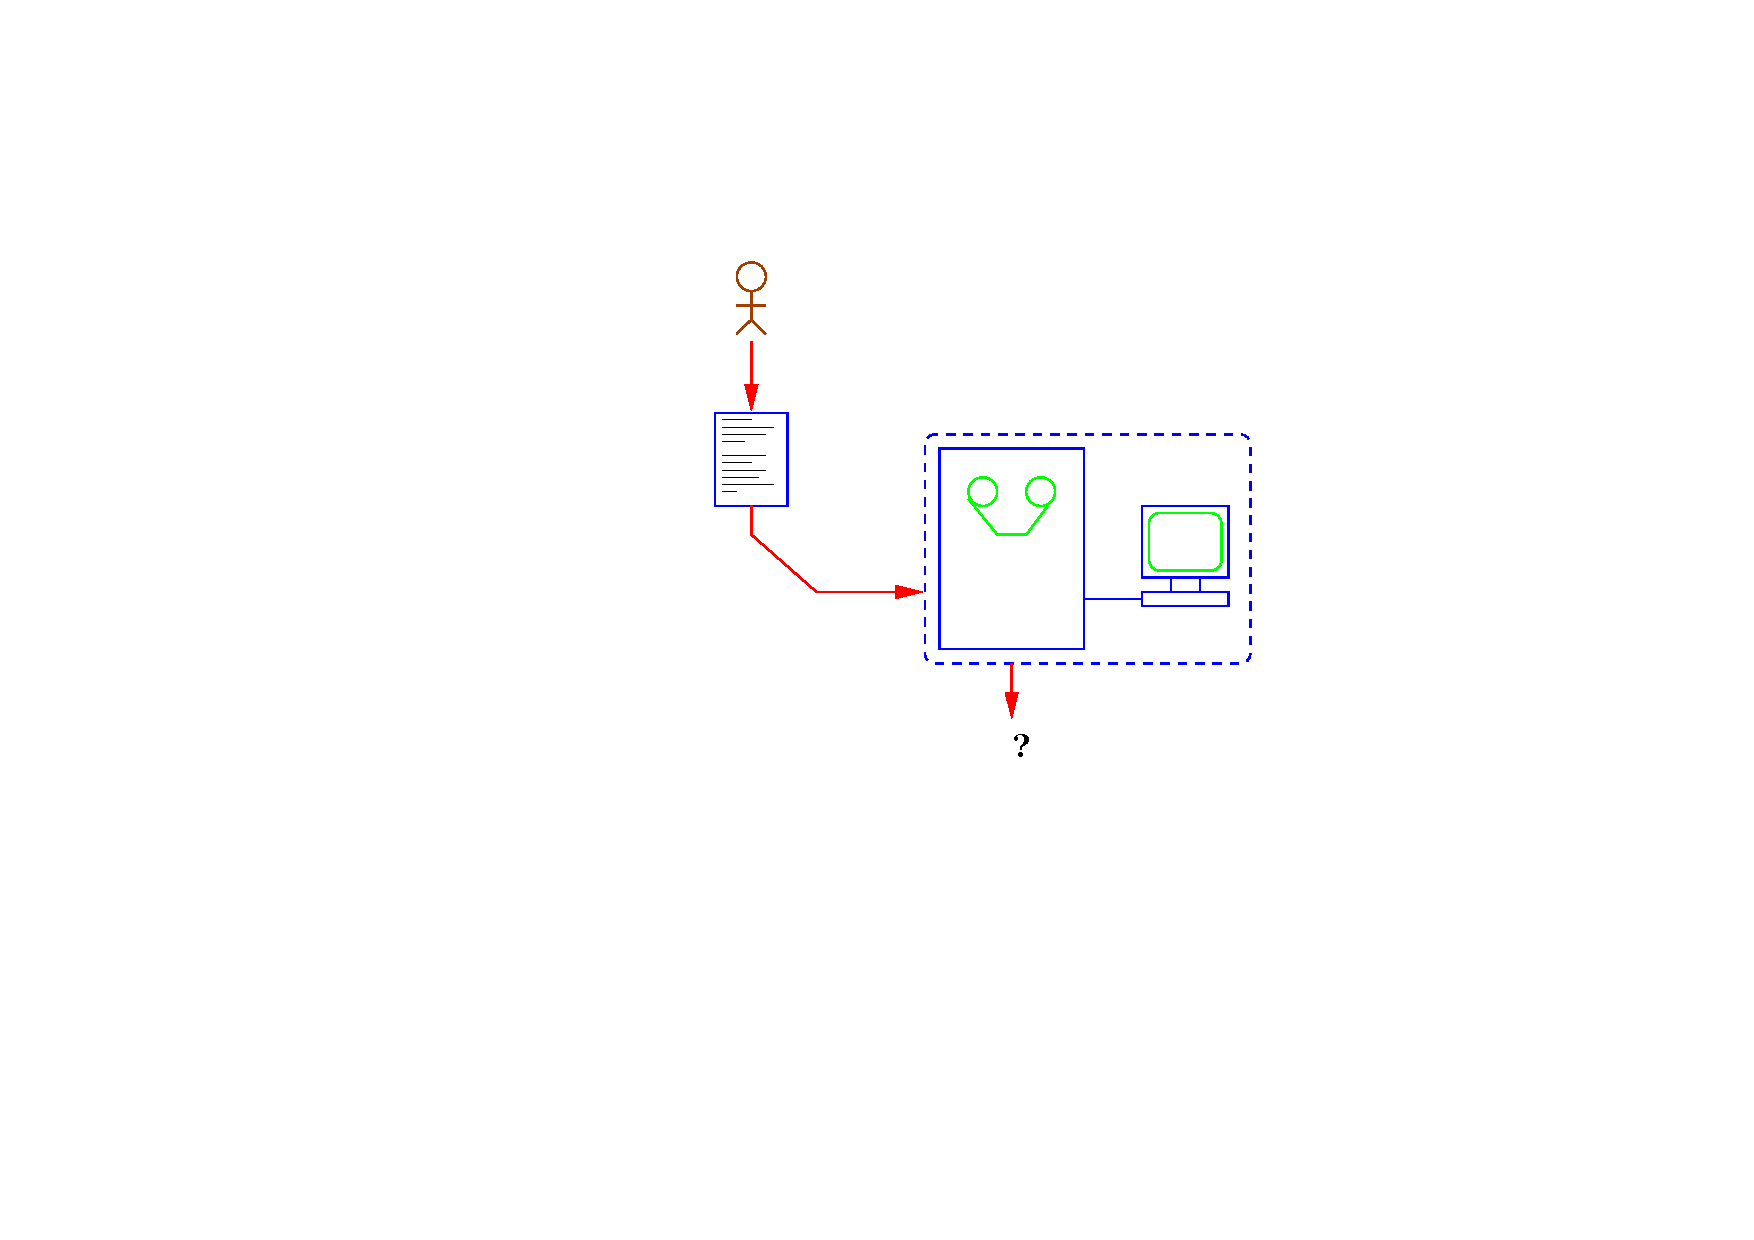
\includegraphics[scale=0.5]{img/imagine1}
\end{center}
\vspace{-.5cm}
\begin{itemize}
	\item Pentru anumite metode de programare (e.g., {\color{red} imperativ\u a, orientat\u a pe obiecte}), nu este u\c sor s\u a stabilim c\u a un program este \intens{corect} sau s\u a \^\i n\c telegem ce \^\i nseamn\u a c\u a este corect (e.g, \^\i n raport cu ce?!). 
	\item \intens{Corectitudinea programelor} devine o problem\u a din ce \^\i n ce mai important\u a, nu doar pentru aplica\c tii "safety-critical".
	\item Avem nevoie de metode ce asigur\u a "calitate", capabile s\u a ofere "garan\c tii".
\end{itemize}
\end{frame}


\begin{frame}[fragile]{C}
\begin{verbatim}
#include <iostream> 
using namespace std;
int main() 
{
  int square; 
  for(int i = 1; i <= 5; ++i)
  { 
    square = i * i;
    cout <<  square << endl; 
  }
}
\end{verbatim}

\begin{itemize}
	\pause \vspace{-.4cm}
	\item \intens{Este corect?} \pause \intens{\^In raport cu ce?}
	\vspace{.2cm}
	\pause
	\item Un \intens{formalism adecvat} trebuie:
	\begin{itemize}
		\item s\u a permit\u a descrierea problemelor (\intens{specifica\c tii}), \c si
		\item s\u a ra\c tioneze despre implementarea lor (\intens{corectitudinea programelor}).
	\end{itemize}
\end{itemize}

\end{frame}

\begin{frame}[fragile]{Care este comportamentul corect?}

\begin{verbatim}
  int main(void) {
    int x = 0;
    return (x = 1) + (x = 2);
  }
\end{verbatim}
\onslide<2>
Conform standardului C, comportamentul programului este \structure{nedefinit}.
\begin{itemize}
\item GCC4, MSVC: valoarea întoarsă e \alert{4}
\item GCC3, ICC, Clang: valoarea întoarsă e \alert{3}
\end{itemize}
\end{frame}

\begin{frame}[fragile]{Care este comportamentul corect?}

\begin{verbatim}
  int r; 
  int f(int x) {
    return (r = x);
  }
  int main() {
    return f(1) + f(2), r;
  }
\end{verbatim}

\onslide<2> Conform standardului C, comportamentul programului este \structure{corect}, dar \structure{subspecificat}:\\
poate întoarce atât valoarea \alert{1} cât și \alert{2}.
\end{frame}

%-------------------------------------------------------------
\begin{frame}{ Tipuri de semantic\u a}

Semantica d\u a \intens{"\^\i n\c teles"} unui program.
\medskip \pause
\begin{itemize}
	\item \intens{Opera\c tional\u a:}
	\begin{itemize}
		\item \^In\c telesul programului este definit \^\i n func\c tie de pa\c sii (transform\u ari dintr-o stare \^\i n alta) care apar \^\i n timpul execu\c tiei.
	\end{itemize}
	\medskip \pause
	\item \intens{Denota\c tional\u a:}
	\begin{itemize}
		\item \^In\c telesul programului este definit abstract ca element dintr-o structur\u a matematic\u a adecvat\u a.
	\end{itemize}
	\medskip \pause
	\item \intens{Axiomatic\u a:}
	\begin{itemize}
		\item \^In\c telesul programului este definit indirect \^\i n func\c tie de axiomele \c si regulile  pe care le verific\u a.
	\end{itemize}
	\medskip \pause
	\item \intens{Statică / a tipurilor}
	\begin{itemize}
		\item Reguli de bună-formare pentru programe
		\item Oferă garanții privind execuția (e.g., nu se blochează)
	\end{itemize}
	
	\end{itemize}
	
%\medskip \pause	
%\begin{center}
%{\color{red} La acest curs, vom defini un limbaj \c si semantica lui folosind Prolog.}
%\end{center}

\end{frame}


\subsection{Bazele programării funcționale / logice}\subsectionframe

%-------------------------------------------------------------
\begin{frame}{Principalele paradigme de programare}
\begin{itemize}
	\item \intens{Imperativ\u a} (\intens{\underline{cum}} calcul\u am)
	\vspace{.2cm}
	\begin{itemize}
	\item \intens{Procedural\u a}
		\vspace{.2cm}
	\item \intens{Orientat\u a pe obiecte}
	
	\end{itemize}
	
	\vspace{.5cm}
	\item  \intens{Declarativ\u a} (\intens{\underline{ce}} calcul\u am)
		\vspace{.2cm}
	\begin{itemize}
	
	\item \intens{Logic\u a}
	\vspace{.2cm}
	\item \intens{Func\c tional\u a}

	\end{itemize}

	\begin{block}{Fundamentele paradigmelor de programare}
		\begin{description}
			\item[Imperativă] Execuția unei Mașini Turing
			\item[Funcțională] Beta-reducție în Lambda Calcul
			\item[Logică] Rezoluția în logica clauzelor Horn
		\end{description}
	\end{block}

\end{itemize}

% \pause
%\begin{center}
%{\color{red} La acest curs, ve\c ti inv\u a\c ta \\  programare logic\u a.}
%\end{center}
\end{frame}

%-------------------------------------------------------------

\begin{frame}{Programare declarativ\u a}

	\begin{itemize}
		\item Programatorul spune \intens{ce} vrea s\u a calculeze, dar nu specific\u a concret \intens{cum} calculeaz\u a.
		\medskip
		\item Este treaba interpretorului (compilator/implementare) s\u a identifice cum s\u a efectueze calculul respectiv.
		\medskip
		\item Tipuri de programare declarativ\u a:
		\begin{itemize}
			\item Programare func\c tional\u a (e.g., Haskell)
			\item Programare logic\u a (e.g., Prolog)
			\item Limbaje de interogare (e.g., SQL)
			
		\end{itemize}
	\end{itemize}
\end{frame}

\begin{frame}{Programare funcțională}
	\begin{description}
		\vfill\item[Esență:] funcții care relaționează intrările cu ieșirile
		\vfill\item[Caracteristici:]
		\begin{itemize}
			\item funcții de ordin înalt -- funcții parametrizate de funcții
			\item grad înalt de abstractizare (e.g., functori, monade)
			\item grad înalt de reutilizarea codului --- polimorfism
		\end{itemize}
		\vfill\item[Fundamente:]
		\begin{itemize}
			\item Teoria funcțiilor recursive
			\item Lambda-calcul ca model de computabilitate (echivalent cu mașina Turing)
		\end{itemize}
		\vfill\item[Inspirație:]
		\begin{itemize}
			\item Inferența tipurilor pentru templates/generics in POO
			\item Model pentru programarea distribuită/bazată pe evenimente (callbacks)
		\end{itemize}
	\end{description}
\end{frame}

%-------------------------------------------------------------
\begin{frame}{Programare logic\u a}


\begin{itemize}
	\item \intens{Programarea logic\u a} este o paradigm\u a de programare \\
	bazat\u a pe logic\u a formal\u a.
	
	\vspace{.2cm} \pause
	\item Unul din sloganurile program\u arii logice:
	\begin{center}
	\href{https://www.doc.ic.ac.uk/~rak/papers/History.pdf}{\intens{\textbf{Program = Logic\u a + Control}}}  \quad {\em (R. Kowalski)}	
	\end{center} 
	
	\vspace{.2cm} \pause
	\item Programarea logic\u a poate fi privit\u a ca o deduc\c tie controlat\u a.	
	
	\vspace{.2cm} \pause
	\item Un \intens{program} scris \^\i ntr-un limbaj de programare logic\u a este
	\begin{center}
	\intens{o list\u a de formule \^\i ntr-o logic\u a}
	\end{center}
	ce exprim\u a fapte \c si reguli despre o problem\u a.

	\vspace{.2cm} \pause
	\item Exemple de limbaje de programare logic\u a: 
		\begin{itemize}
			\item \intens{Prolog}
			\item \intens{Answer set programming (ASP)}
			\item \intens{Datalog}
		\end{itemize}
\end{itemize}
\end{frame}


%---------------------------------------------------------------------
%\begin{frame}
%\vspace{1cm}
%\begin{figure}[h]
 % \centering
 %   
\includegraphics[width=0.6\textwidth]{img/work}
%\end{figure}
%\end{frame}


%-------------------------------------------------------------
\section{Programare logic\u a \& Prolog} \sectionframe
%-------------------------------------------------------------



%---------------------------------------------------------------------
\begin{frame}{Programare logic\u a - \^\i n mod idealist}
\begin{itemize}
	\item Un \intens{"program logic"} este o colec\c tie de propriet\u a\c ti presupuse (sub form\u a de formule logice) despre lume (sau mai degrab\u a despre lumea programului).
	\medskip
	\item Programatorul furnizeaz\u a \c si o proprietate (o formula logic\u a) care poate s\u a fie sau nu adev\u arat\u a \^\i n lumea respectiv\u a (\intens{\^\i ntrebare, {\em query}}).
	\medskip
	\item Sistemul determin\u a dac\u a proprietatea aflat\u a sub semnul \^\i ntreb\u arii este o consecin\c t\u a a propriet\u a\c tilor presupuse \^\i n program.
	\medskip
		\item Programatorul nu specific\u a metoda prin care sistemul verific\u a dac\u a \^\i ntrebarea este sau nu consecin\c t\u a a programului.
\end{itemize}
\end{frame}
%---------------------------------------------------------------------

%---------------------------------------------------------------------
%\begin{frame}{Programare logic\u a - \^\i n mod idealist}
%\intens{Aspecte declarative} ale program\u arii logice:
%\begin{itemize}
%	\item Programatorul nu specific\u a metoda prin care sistemul %verific\u a dac\u a \^\i ntrebarea este sau nu consecin\c t\u a a %programului.
%	\medskip
%	\item Faptul c\u a \^\i ntrebarea chiar este sau nu consecin\c t%\u a este independent de metoda aleas\u a de sistem.
%\end{itemize}
%\end{frame}
%---------------------------------------------------------------------



%---------------------------------------------------------------------
\begin{frame}{Exemplu de program logic}
\begin{center}
\begin{tabular}{rcl}
\texttt{oslo} & $\to$ & \texttt{windy} \\[.5em]
\texttt{oslo} & $\to$ & \texttt{norway} \\[.5em]
\texttt{norway} & $\to$ & \texttt{cold} \\[.5em]
\texttt{cold $\wedge$ windy} & $\to$ & \texttt{winterIsComing} \\[.5em]
& & \texttt{oslo}\\
\end{tabular}
\end{center}
\bigskip\pause

\begin{block}{Exemplu de \^\i ntrebare}
\begin{center}
Este adev\u arat \intens{\texttt{winterIsComing}}?
\end{center}
\end{block}
\end{frame}
%---------------------------------------------------------------------

%---------------------------------------------------------------------

\begin{frame}{Prolog}

\vfill\begin{itemize}
	\item bazat pe logica clauzelor Horn
	\item semantica opera\c tional\u a este bazat\u a pe rezolu\c tie
	\item este Turing complet
%	\item vom folosi implementarea \intens{SWI-Prolog}
%	\item vom folosi varianta online \intens{SWISH} a SWI-Prolog
%	\begin{itemize}
%		\item \underline{\url{http://swish.swi-prolog.org/}}
%	\end{itemize}
\end{itemize}
\pause\vfill

\begin{block}{}
Limbajul Prolog este folosit pentru programarea sistemului IBM Watson!
\begin{center}

\includegraphics[scale=0.05]{img/watson}
\end{center}
Pute\c ti citi mai multe detalii   \href{https://www.cs.nmsu.edu/ALP/2011/03/natural-language-processing-with-prolog-in-the-ibm-watson-system/}{\intens{aici}}.
\end{block}

\end{frame}


%---------------------------------------------------------------------
%\begin{frame}{Exemplu de \^\i ntrebare}

%\begin{center}
%Este adev\u arat \intens{\texttt{winterIsComing}}?
%\end{center}

%\medskip
%\begin{figure}[h]
%  \centering
%    
\includegraphics[width=0.6\textwidth]{img/winter}
%\end{figure}

%\end{frame}

%---------------------------------------------------------------------
\begin{frame}{Exemplul de mai sus în SWI-Prolog}
\intens{Program:}
\begin{alltt}
windy :- oslo. \\
norway :- oslo. \\
cold :- norway. \\
winterIsComing :- windy, cold. \\
oslo. \\
\end{alltt}

\bigskip
\intens{Intrebare:}
\begin{alltt}
?- winterIsComing.\\
true
\end{alltt}

\bigskip
\underline{\url{http://swish.swi-prolog.org/}}
\end{frame}
%---------------------------------------------------------------------
%---------------------------------------------------------------------
%\begin{frame}{Sintax\u a: constante, variabile, termeni compu\c si}
%
%\bigskip
%
%\begin{itemize}
%	
%		
%		  \item \intens{Atomi}: \texttt{sansa, 'Jon Snow', 
%		  jon\_snow}
%		  \bigskip
%		  \item \intens{Numere}: \texttt{23, 23.03,-1}
%		
%		\medskip
%		
%		\intens{Atomii} \c si \intens{numerele} sunt \intens{constante}.
%		\medskip
%		\item \intens{Variabile}: \texttt{X, Stark, \_house}
%
%		\bigskip
%			\item Termeni \intens{compu\c si}: \texttt{father(eddard, jon\_snow)},
%			
%\hspace*{1cm}\texttt{and(son(bran,eddard), daughter(arya,eddard))}
%
%\begin{itemize}
%\item[-]   forma general\u a:	\intens{atom(termen,$\ldots$, termen)}
% \item[-]  atom-ul care denume\c ste termenul se nume\c ste \intens{functor}		      	
%			      	
%\item[-] num\u arul de argumente se nume\c ste \intens{aritate}			      	\end{itemize}
%\end{itemize}
%
%\begin{center}
%
\includegraphics[scale=.2]{img/building-blocks}
%\end{center}
%\end{frame}
%
%
%%---------------------------------------------------------------------
%\begin{frame}{Un mic exerci\c tiu sintactic}
%
%Care din urm\u atoarele \c siruri de caractere sunt \intens{constante} \c si care sunt \intens{variabile} \^\i n Prolog?
%
%\begin{itemize}
%	\item vINCENT \onslide<2->{-- \intens{constant\u a}}
%	\item Footmassage \onslide<2->{-- \myalert{variabil\u a}} 
%	\item variable23 \onslide<2->{-- \intens{constant\u a}}
%	\item Variable2000 \onslide<2->{-- \myalert{variabil\u a}} 
%	\item big\_kahuna\_burger \onslide<2->{-- \intens{constant\u a}}
%	\item 'big  kahuna  burger' \onslide<2->{-- \intens{constant\u a}}
%	\item big  kahuna  burger \onslide<2->{-- \alert{nici una, nici alta}}
%	\item 'Jules' \onslide<2->{-- \intens{constant\u a}}
%	\item \_Jules \onslide<2->{-- \myalert{variabil\u a}} 
%	\item '\_Jules' \onslide<2->{-- \intens{constant\u a}}
%\end{itemize}
%
%\end{frame}
%
%%---------------------------------------------------------------------
%\begin{frame}[fragile]{Program \^{\i}n Prolog = baz\u a de cuno\c stin\c te}
%
%\begin{example}
%Un program \^\i n Prolog:
%\begin{columns}
%\begin{column}{.5\textwidth}
%\begin{verbatim}
%father(eddard,sansa). 
%father(eddard,jon_snow).
%
%mother(catelyn,sansa). 
%mother(wylla,jon_snow).
%
%stark(eddard).
%stark(catelyn).
%
%stark(X) :- father(Y,X),  stark(Y).
%\end{verbatim}
%\end{column}
%\begin{column}{.3\textwidth}
%
\includegraphics[scale=.8]{img/Stark.png}
%\end{column}
%\end{columns}
%\smallskip
%\end{example}
%\medskip
%
%Un program \^{\i}n Prolog este o \intens{baz\u a de cuno\c stin\c te} (\intens{K}nowledge \intens{B}ase).
%\end{frame}
%
%%---------------------------------------------------------------------
%
%\begin{frame}[fragile]{Program \^{\i}n Prolog = mul\c time de predicate}
%
%Practic, g\^{a}ndim un program \^{\i}n Prolog ca o mul\c time de \intens{predicate}  cu ajutorul c\u arora descriem {\it lumea} ({\it universul}) programului respectiv.
% 
%\begin{example}
%\begin{columns}
%\begin{column}{.5\textwidth}
%\begin{verbatim}
%father(eddard,sansa). 
%father(eddard,jon_snow).
%
%mother(catelyn,sansa). 
%mother(wylla,jon_snow).
%
%stark(eddard).
%stark(catelyn).
%
%stark(X) :- father(Y,X),  stark(Y).
%\end{verbatim}
%\end{column}
%\begin{column}{.3\textwidth}
%\intens{\textbf{Predicate:}}\\
%\intens{father/2}\\
%\intens{mother/2}\\
%\intens{stark/1}
%\end{column}
%\end{columns}
%\smallskip
%\end{example}
%
%
%
%\end{frame}
%%----------------------------------------------------
%
%
%\begin{frame}{Un program \^\i n Prolog}
%
%\begin{center}
%%Un program \^\i n Prolog r\u aspunde la \^\i ntreb\u ari.
%
%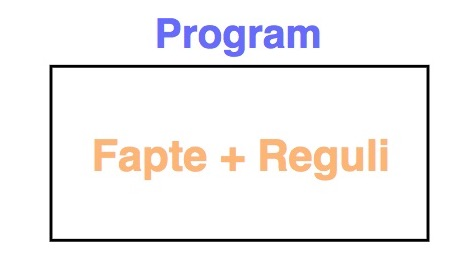
\includegraphics[scale=.3]{img/Prolog1}
%
%
%\end{center}
%
%
%\end{frame}
%%---------------------------------------------------------------------
%
%
%%---------------------------------------------------------------------
%\begin{frame}{Program }
%
%\begin{itemize}
%	\item Un \intens{program} \^\i n Prolog este format din \intens{reguli} de forma
%	\begin{center}
%	\intens{\texttt{Head :- Body.}}
%	\end{center} 
%	\medskip
%	
%\item \intens{Head} este un predicat, iar \intens{Body} este o secven\c t\u a de predicate separate prin virgul\u a.
%
%\medskip
%	
%\item Regulile f\u ar\u a \texttt{Body} se numesc \intens{fapte}.
%\end{itemize}
%
%\medskip \pause
%\begin{example}
%\begin{itemize}
%	\item  Exemplu de regul\u a: \texttt{stark(X) :- father(Y,X), stark(Y).}
%	\item  Exemplu de fapt: \texttt{father(eddard, jon\_snow)}.
%\end{itemize}
%\end{example}
%\end{frame}
%%---------------------------------------------------------------------
%
%
%\begin{frame}{Interpretarea din punctul de vedere al logicii}
%\vspace*{0.3cm}
%
%\begin{itemize}
%\item operatorul \intens{\textbf{:-}} este implica\c tia logic\u a
% \intens{$\leftarrow$}
%\begin{example}
%\texttt{winterfell(X) :- stark(X)}
%\smallskip
%
%\intens{dac\u a} \texttt{stark(X)} \intens{este adev\u arat, atunci} 
%\texttt{winterfell(X)} \intens{este adev\u arat.}
%\end{example}
%\pause
%
%\item virgula \intens{,} este conjunc\c tia \intens{$\wedge$}
%
%\begin{example}
%\texttt{stark(X) :- father(Y,X), stark(Y)}
%
%\smallskip
%
%\intens{dac\u a} \texttt{father(Y,X)} \intens{\c si} \texttt{stark(Y)}  \intens{sunt adev\u arate,}
%
%\intens{atunci} \texttt{stark(X)} \intens{este adev\u rat.}
%\end{example}
%\end{itemize}
%\end{frame}
%
%\begin{frame}{Interpretarea din punctul de vedere al logicii}
%\begin{itemize}
%\item  mai multe reguli cu \intens{acela\c si \texttt{Head}} definesc acela\c si predicat, \^{\i}ntre defi\c tii fiind un \intens{sau} logic. 
%\end{itemize}
%
%\begin{example}
%\begin{alltt}
%got\_house(X) :- stark(X).\\
%got\_house(X) :- lannister(X).\\
%got\_house(X) :- targaryen(X).\\
%got\_house(X) :- baratheon(X).
%\end{alltt}
%\smallskip
%
%\intens{dac\u a} 
%
% \texttt{stark(X)} \intens{este adev\u arat sau}
%
% \texttt{lannister(X)} \intens{este adev\u arat sau}
% 
%  \texttt{targaryen(X)} \intens{este adev\u arat sau}
% 
%  \texttt{baratheon(X)}  \intens{este adev\u arat,}
%  
%\intens{ atunci} 
%
%\texttt{got\_house(X)} \intens{este adev\u arat}.
%
%
%
%\end{example}
%\end{frame}
%
%%---------------------------------------------------------------------
%
%\begin{frame}{Un program \^\i n Prolog}
%
%\begin{center}
%%Un program \^\i n Prolog r\u aspunde la \^\i ntreb\u ari.
%
%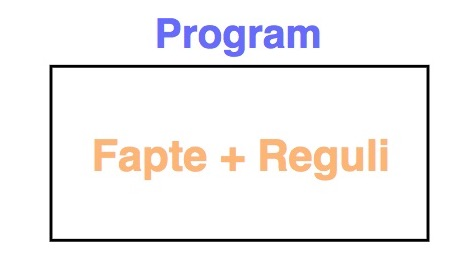
\includegraphics[scale=.3]{img/Prolog1}
%
%\vspace*{1cm}
%
%Cum folosim un program \^{\i}n Prolog?
%\end{center}
%
%
%\end{frame}
%%---------------------------------------------------------------------
%
%\begin{frame}{\^Intreb\u ari \^\i n Prolog}
%
%\begin{center}
%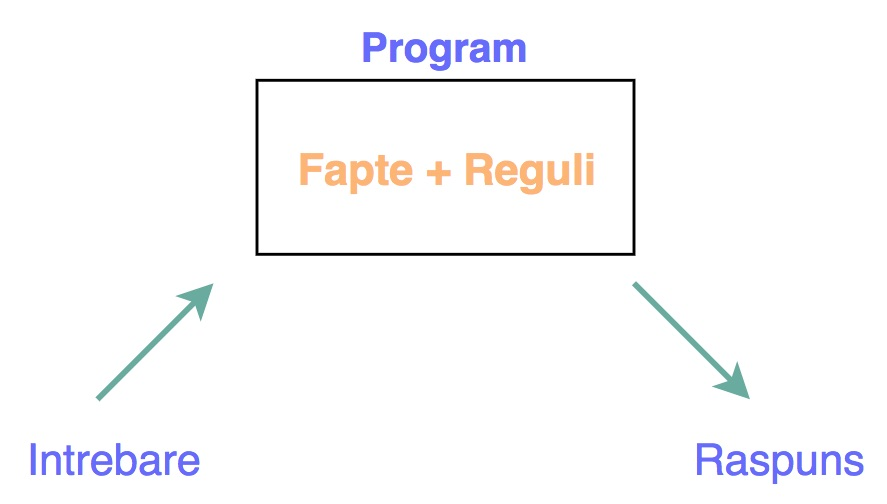
\includegraphics[scale=.3]{img/Prolog}
%\end{center}
%
%\end{frame}
%%---------------------------------------------------------------------
%
%%---------------------------------------------------------------------
%
%\begin{frame}{\^Intreb\u ari \c si \c tinte \^\i n Prolog}
%
%\begin{itemize}
%	\item Prolog poate r\u aspunde la \^\i ntreb\u ari legate de consecin\c tele rela\c tiilor descrise \^\i ntr-un program \^\i n Prolog.
%	\smallskip
%	\item \intens{\^Intreb\u arile} sunt de forma:
%	\begin{center}
%	\intens{\texttt{?- predicat$_1$($\ldots$),$\ldots$,predicat$_n$($\ldots$).}}
%	\end{center}
%	\smallskip
%	\item Prolog verific\u a dac\u a \^\i ntrebarea este o consecin\c t\u a a rela\c tiilor definite \^\i n program.
%	\smallskip
%	\item Dac\u a este cazul, Prolog caut\u a valori pentru variabilele care apar \^\i n \^\i ntrebare astfel \^\i nc\^at \^\i ntrebarea s\u a fie o consecin\c t\u a a rela\c tiilor din program.
%\smallskip	
%	\item un predicat care este analizat pentru a se r\u aspunde la o \^{\i}ntrebare se nume\c ste \intens{\c tint\u a} (\intens{goal}).
%\end{itemize}
%\end{frame}
%%---------------------------------------------------------------------
%
%%---------------------------------------------------------------------
%
%\begin{frame}{\^Intreb\u ari \^\i n Prolog}
%
%
%Prolog poate da 2 tipuri de r\u aspunsuri:
%	\begin{itemize}
%		\item {\color{red} \texttt{false}} -- \^\i n cazul \^\i n care \^\i ntrebarea nu este o consecin\c t\u a a programului.
%		\smallskip
%		\item \intens{\texttt{true}} sau \intens{valori pentru variabilele din \^\i ntrebare} \^\i n cazul \^\i n care \^\i ntrebarea este o consecin\c t\u a a programului.
%	\end{itemize}
%
%\pause
%\begin{example}
%\smallskip
%\begin{columns}
%\begin{column}{.4\textwidth}
% \texttt{?- stark(jon\_snow)} \\
%	  \texttt{true}
%	  
%\texttt{?- stark(wylla)} \\
%	  \texttt{false}
%\vspace{.8cm}	
%\end{column}
%\begin{column}{.4\textwidth}
%\texttt{?- stark(X)} \\
%	\texttt{X = eddard ;} \\
%	\texttt{X = catelyn ;} \\
%	\texttt{X = sansa ;} \\
%	\texttt{X = jon\_snow ;} \\
%	\texttt{false} \\
%\end{column}
%\end{columns}
%\smallskip
%\end{example}
%\end{frame}
%
%
%%---------------------------------------------------------------------
%
%
%
%
%%---------------------------------------------------------------------
%
%\begin{frame}[fragile]{Cum g\u ase\c ste Prolog r\u aspunsul}
%
%Pentru a g\u asi un raspuns, \intens{Prolog \^\i ncearc\u a regulile \^\i n ordinea apari\c tiei lor.}
%
%\medskip 
%\begin{example}
%
%S\u a presupunem c\u a avem programul: 
%\begin{verbatim}
%foo(a).  foo(b).  foo(c).
%\end{verbatim}
%\c si c\u a punem urm\u atoarea \^\i ntrebare: \\
%{\color{blue}\texttt{?- foo(X).}}\\
%{\color{blue}\texttt{X = a.}}\\
%\end{example}
%
%Pentru a r\u aspunde la \^{\i}ntrebare se caut\u a o \intens{potrivire} (\intens{unificator}) \^{\i}ntre scopul {\color{blue}\texttt{foo(X)}} \c si baza de cuno\c stin\c te. Raspunsul este \intens{substitu\c tia} care realizeaz\u a potrivirea, \^{\i}n cazul nostru {\color{blue}\texttt{X = a}}. 
%
%\begin{center}
%\intens{Vom discuta detaliat algoritmul de unificare!}
%\end{center}
%
%\end{frame}
%
%
%%---------------------------------------------------------------------
%
%\begin{frame}[fragile]{Cum g\u ase\c ste Prolog r\u aspunsul}
%
%Pentru a g\u asi un raspuns, \intens{Prolog \^\i ncearc\u a regulile \^\i n ordinea apari\c tiei lor.}
%
%\medskip 
%\begin{example}
%
%S\u a presupunem c\u a avem programul: 
%\begin{verbatim}
%foo(a).  foo(b).  foo(c).
%\end{verbatim}
%\c si c\u a punem urm\u atoarea \^\i ntrebare: \\
%{\color{blue}\texttt{?- foo(X).}}\\
%{\color{blue}\texttt{X = a.}}\\
%\medskip
%
%{\color{blue}\texttt{?- foo(d).}}\\
%{\color{red}\texttt{false}}\\
%\smallskip
%\end{example}
%
%Daca\u a nu se poate face potrivirea, r\u aspunsul este 
%{\color{red}{false}}.
%
%\end{frame}
%%---------------------------------------------------------------------
%
%\begin{frame}[fragile]{Cum g\u ase\c ste Prolog r\u aspunsul}
%
%Pentru a g\u asi un raspuns, \intens{Prolog \^\i ncearc\u a regulile \^\i n ordinea apari\c tiei lor.}
%
%\medskip 
%\begin{example}
%
%S\u a presupunem c\u a avem programul: 
%\begin{verbatim}
%foo(a).  foo(b).  foo(c).
%\end{verbatim}
%\c si c\u a punem urm\u atoarea \^\i ntrebare: \\
%{\color{blue}\texttt{?- foo(X).}}\\
%{\color{blue}\texttt{X = a.}}\\
%
%\smallskip\pause
%
%Dac\u a dorim mai multe r\u aspunsuri, tast\u am \color{blue}{\texttt{;}}\\
%\smallskip
%
%{\color{blue}\texttt{?- foo(X).}}\\
%{\color{blue}\texttt{X = a ;}}\\
%{\color{blue}\texttt{X = b ;}}\\
%{\color{blue}\texttt{X = c.}}
%
%
%\end{example}
%
%\end{frame}
%
%\addtocounter{framenumber}{-1}
%%------------------------------------------------------------------
%\begin{frame}[fragile]{Cum g\u ase\c ste Prolog r\u aspunsul}
%
%Pentru a g\u asi un raspuns, \intens{Prolog \^\i ncearc\u a regulile \^\i n ordinea apari\c tiei lor.}
%
%\medskip
%\begin{example}
%\begin{multicols}{2}
%S\u a presupunem c\u a avem programul: 
%\begin{verbatim}
%foo(a). 
%foo(b). 
%foo(c).
%\end{verbatim}
%\c si c\u a punem urm\u atoarea \^\i ntrebare: \\
%{\color{blue}\texttt{?- foo(X).}}
%\columnbreak
%\begin{figure}[h]
%    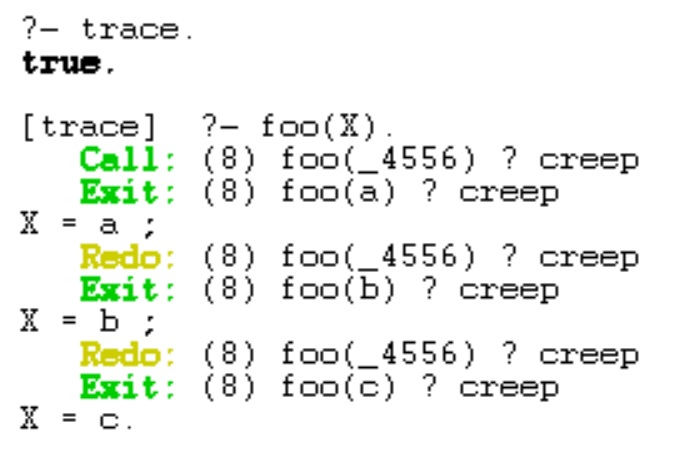
\includegraphics[width=0.4\textwidth]{prolog/trace1}
%\end{figure}
%\end{multicols}
%\end{example}
%\end{frame}
%
%%------------------------------------------------------------------
%
%\begin{frame}[fragile]{Cum g\u ase\c ste Prolog r\u aspunsul}
%
%Pentru a g\u asi un raspuns, \intens{Prolog redenume\c ste variabilele.}
%
%\medskip 
%\begin{example}
%\begin{multicols}{2}
%S\u a presupunem c\u a avem programul: 
%\begin{verbatim}
%foo(a). 
%foo(b). 
%foo(c).
%\end{verbatim}
%\c si c\u a punem urm\u atoarea \^\i ntrebare: \\
%{\color{blue}\texttt{?- foo(X).}}
%\columnbreak
%\begin{figure}[h]
%    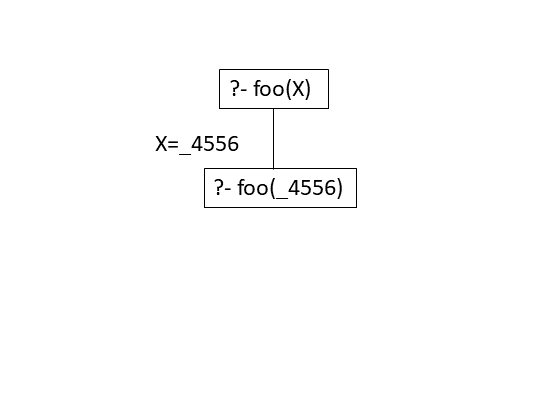
\includegraphics[width=0.4\textwidth]{prolog/foo1}
%\end{figure}
%\end{multicols}
%\end{example}
%
%
%
%\end{frame}
%
%\addtocounter{framenumber}{-1}
%%------------------------------------------------------------------
%\begin{frame}[fragile]{Cum g\u ase\c ste Prolog r\u aspunsul}
%
%
%Pentru a g\u asi un raspuns, \intens{Prolog \^\i ncearc\u a regulile \^\i n ordinea apari\c tiei lor.}
%
%\medskip
%\begin{example}
%\begin{multicols}{2}
%S\u a presupunem c\u a avem programul: 
%\begin{verbatim}
%foo(a). 
%foo(b). 
%foo(c).
%\end{verbatim}
%\c si c\u a punem urm\u atoarea \^\i ntrebare: \\
%{\color{blue}\texttt{?- foo(X).}}
%\columnbreak
%\begin{figure}[h]
%    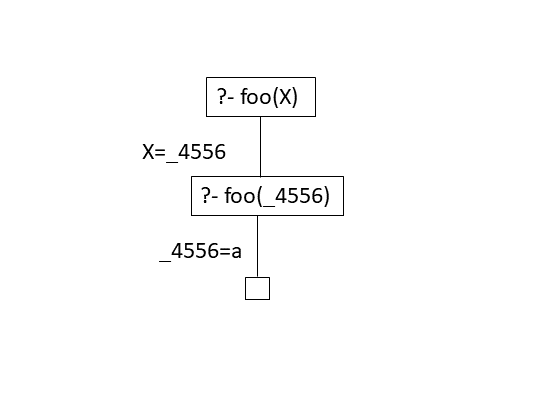
\includegraphics[width=0.4\textwidth]{prolog/foo2}
%\end{figure}
%\end{multicols}
%\end{example}
%\medskip
%
%\^{I}n acest moment, a fost g\u asit\u a  prima solu\c tie: \texttt{X=\_4556=a}.
%\end{frame}
%
%\addtocounter{framenumber}{-1}
%%------------------------------------------------------------------
%\begin{frame}[fragile]{Cum g\u ase\c ste Prolog r\u aspunsul}
%
%Pentru a g\u asi un raspuns, \intens{Prolog \^\i ncearc\u a clauzele \^\i n ordinea apari\c tiei lor.}
%
%\medskip
%\begin{example}
%\begin{multicols}{2}
%S\u a presupunem c\u a avem programul: 
%\begin{verbatim}
%foo(a). 
%foo(b). 
%foo(c).
%\end{verbatim}
%\c si c\u a punem urm\u atoarea \^\i ntrebare: \\
%{\color{blue}\texttt{?- foo(X).}}
%\columnbreak
%\begin{figure}[h]
%    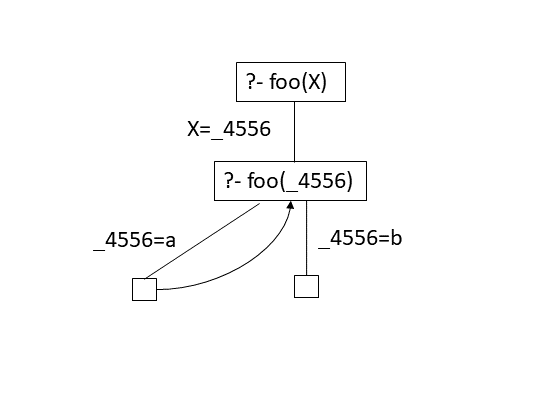
\includegraphics[width=0.4\textwidth]{prolog/foo3}
%\end{figure}
%\end{multicols}
%\end{example}
%\medskip
%
%Dac\u a se dore\c ste \^{\i}nc\u a un r\u aspuns, atunci se face un pas \^{\i}napoi \^{\i}n \intens{arborele de c\u autare} \c si se \^{\i}ncearc\u a satisfacerea \c tintei cu o nou\u a valoare.
%\end{frame}
%
%\addtocounter{framenumber}{-1}
%%------------------------------------------------------------------
%\begin{frame}[fragile]{Cum g\u ase\c ste Prolog r\u aspunsul}
%
%Pentru a g\u asi un raspuns, \intens{Prolog \^\i ncearc\u a clauzele \^\i n ordinea apari\c tiei lor.}
%
%\medskip
%\begin{example}
%\begin{multicols}{2}
%S\u a presupunem c\u a avem programul: 
%\begin{verbatim}
%foo(a). 
%foo(b). 
%foo(c).
%\end{verbatim}
%\c si c\u a punem urm\u atoarea \^\i ntrebare: \\
%{\color{blue}\texttt{?- foo(X).}}
%\columnbreak
%\begin{figure}[h]
%    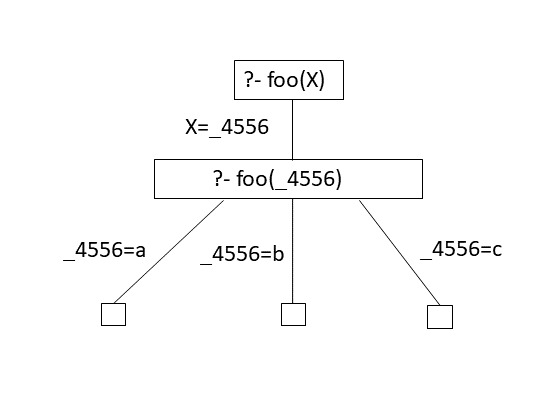
\includegraphics[width=0.4\textwidth]{prolog/foo4}
%
%\begin{center}
%\intens{arborele de c\u autare}
%\end{center}
%\end{figure}
%\end{multicols}
%\end{example}
%
%\end{frame}
%
%
%%-------------------------------------------------------------------
%
%%------------------------------------------------------------------
%\begin{frame}[fragile]{Cum g\u ase\c ste Prolog r\u aspunsul}
%
%\medskip 
%
%\begin{example}
%\begin{multicols}{2}
%S\u a presupunem c\u a avem programul: 
%\begin{verbatim}
%bar(b). 
%bar(c). 
%
%baz(c).
%\end{verbatim}
%\c si c\u a punem urm\u atoarea \^\i ntrebare: \\
%{\color{blue}\texttt{?- bar(X),baz(X).}}
%\columnbreak
%\begin{figure}[h]
%    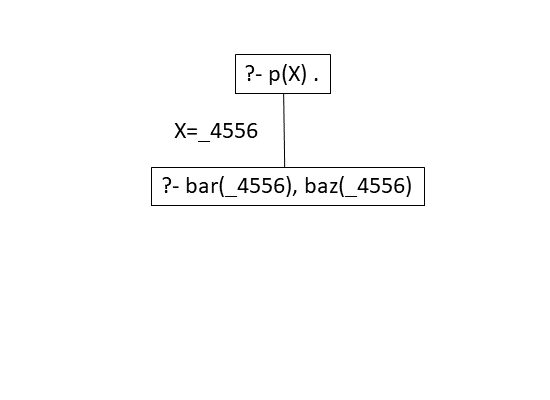
\includegraphics[width=0.4\textwidth]{prolog/bar1}
%\end{figure}
%\end{multicols}
%\end{example}
%\end{frame}
%
%\addtocounter{framenumber}{-1}
%%------------------------------------------------------------------
%\begin{frame}[fragile]{Cum g\u ase\c ste Prolog r\u aspunsul}
%
%\medskip
%\intens{Prolog se \^\i ntoarce la ultima alegere dac\u a o sub-\c tint\u a e\c sueaz\u a.}
%
%\medskip
%\begin{example}
%\begin{multicols}{2}
%S\u a presupunem c\u a avem programul: 
%\begin{verbatim}
%bar(b). 
%bar(c). 
%baz(c).
%\end{verbatim}
%\c si c\u a punem urm\u atoarea \^\i ntrebare: \\
%{\color{blue}\texttt{?- bar(X),baz(X).}}
%\columnbreak
%\begin{figure}[h]
%    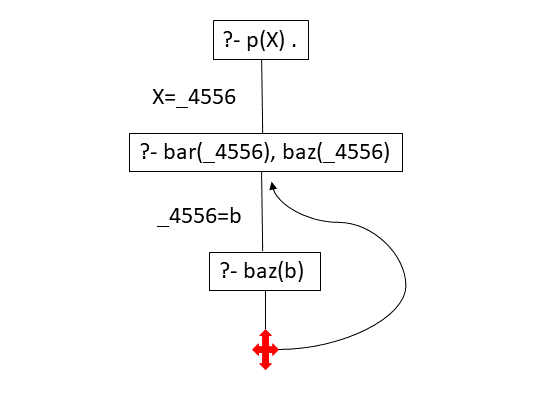
\includegraphics[width=0.4\textwidth]{prolog/bar2}
%\end{figure}
%\end{multicols}
%\end{example}
%\end{frame}
%
%\addtocounter{framenumber}{-1}
%%------------------------------------------------------------------
%\begin{frame}[fragile]{Cum g\u ase\c ste Prolog r\u aspunsul}
%
%\medskip
%\intens{Prolog se \^\i ntoarce la ultima alegere dac\u a o sub-\c tint\u a e\c sueaz\u a.}
%
%\medskip
%\begin{example}
%\begin{multicols}{2}
%S\u a presupunem c\u a avem programul: 
%\begin{verbatim}
%bar(b). 
%bar(c). 
%baz(c).
%\end{verbatim}
%\c si c\u a punem urm\u atoarea \^\i ntrebare: \\
%{\color{blue}\texttt{?- bar(X),baz(X).}}
%\columnbreak
%\begin{figure}[h]
%    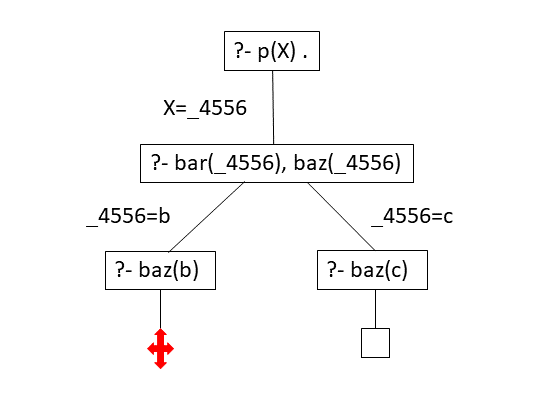
\includegraphics[width=0.4\textwidth]{prolog/bar3}
%\end{figure}
%\end{multicols}
%\end{example}
%\medskip
%
%Solu\c tia g\u asit\u a este: \texttt{X=\_4556=c}.
%\end{frame}
%
%%--------------------------------------------------------------
%
%\begin{frame}[fragile]{Cum g\u ase\c ste Prolog r\u aspunsul}
%
%\medskip
%Ce se \^{\i}nt\^ ampl\u a dac\u a schimb\u am ordinea regulilor?
%
%\medskip
%\begin{example}
%\begin{multicols}{2}
%S\u a presupunem c\u a avem programul: 
%\begin{verbatim}
%bar(c). 
%bar(b). 
%
%baz(c).
%\end{verbatim}
%\c si c\u a punem urm\u atoarea \^\i ntrebare: \\
%{\color{blue}\texttt{?- bar(X),baz(X).}}
%\columnbreak
%\vspace*{0.3cm}
%\end{multicols}
%\end{example}
%\medskip
%
%
%\end{frame}
%
%
%\addtocounter{framenumber}{-1}
%%--------------------------------------------------------------
%
%\begin{frame}[fragile]{Cum g\u ase\c ste Prolog r\u aspunsul}
%
%\medskip
%Ce se \^{\i}nt\^ ampl\u a dac\u a schimb\u am ordinea regulilor?
%
%\medskip
%\begin{example}
%
%S\u a presupunem c\u a avem programul: 
%\begin{verbatim}
%bar(c). 
%bar(b). 
%
%baz(c).
%\end{verbatim}
%\c si c\u a punem urm\u atoarea \^\i ntrebare: \\
%{\color{blue}\texttt{?- bar(X),baz(X).}}\\
%{\color{blue}\texttt{X = c ;}}\\
%{\color{red}\texttt{false}}
%
%\end{example}
%\medskip
%
%V\u a explica\c ti ce s-a \^{\i}nt\^ amplat? Desena\c ti arborele de c\u autare!
%
%\end{frame}
%
%%------------------------------------------------------------------
%\begin{frame}[fragile]{Un program mai complicat}
%\vspace*{0.5cm}
%
%\intens{Problema color\u arii h\u ar\c tilor}
%\smallskip
%
%{\em S\u a se coloreze o hart\u a dat\u a cu un num\u ar minim de culori astfel \^{\i}nc\^{a}t oricare dou\u a \c t\u ari vecine s\u a fie colorate diferit.}  
%
%\medskip
% \onslide<2-3>{\intens{Cum model\u am aceast\u a problem\u a \^{\i}n Prolog?}}
% 
%\begin{example}
%\begin{multicols}{2}
%\onslide<3>{
%Trebuie s\u a definim:
%\begin{itemize}
%\item culorile
%\item harta
%\item constr\^{a}ngerile
%\end{itemize}}
%\columnbreak
%\begin{figure}[h]
%    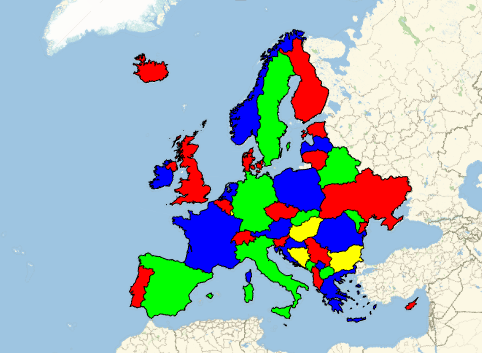
\includegraphics[width=0.4\textwidth]{img/europe1}
%    
%    \href{https://www.wolfram.com/mathematica/new-in-10/entity-based-geocomputation/find-the-shortest-route-through-the-worlds-capital.html}{\footnotesize{\intens{Sursa imaginii}}}
%\end{figure}
%\end{multicols}
%\end{example}
%
%\end{frame}
%
%\setbeamercolor*{block title}{fg=white, bg=MedianLightOrange}
%
%\addtocounter{framenumber}{-1}
%%------------------------------------------------------------------
%\begin{frame}[fragile]{Problema color\u arii h\u ar\c tilor}
%
% \intens{Definim culorile}
%
%\begin{example}
%\vspace{-.3cm}
%\begin{verbatim}
%culoare(albastru).
%culoare(rosu).
%culoare(verde).
%culoare(galben).
%
%\end{verbatim}
%
%
%
%\vspace{2.8cm}
%\end{example}
%
%
%\end{frame}
%
%%---------------------------------------------------------------------
%
%
%
%
%\addtocounter{framenumber}{-1}
%%%------------------------------------------------------------------
%
%%------------------------------------------------------------------
%\begin{frame}[fragile]{Problema color\u arii h\u ar\c tilor}
%
% \intens{Definim culorile, harta}
%
%\begin{example}
%\vspace{-.3cm}
%\begin{verbatim}
%culoare(albastru).
%culoare(rosu).
%culoare(verde).
%culoare(galben).
%\end{verbatim}
%
%\begin{verbatim}
%harta(RO,SE,MD,UA,BG,HU) :- vecin(RO,SE), vecin(RO,UA), 
%                            vecin(RO,MD), vecin(RO,BG),                      	                         
%                            vecin(RO,HU), vecin(UA,MD),
%                            vecin(BG,SE), vecin(SE,HU).
%
%                             
%\end{verbatim}
%
%\vspace{.4cm}
%\end{example}
%\end{frame}
%
%\addtocounter{framenumber}{-1}
%%------------------------------------------------------------------
%\begin{frame}[fragile]{Problema color\u arii h\u ar\c tilor}
%
%\vspace{.4cm}
% \intens{Definim culorile, harta \c si constr\^{a}ngerile.}
% \onslide<2->{\intens{Cum punem \^{\i}ntrebarea?}}
%
%
%\begin{example}
%
%\vspace{-.3cm}
%\begin{verbatim}
%culoare(albastru).
%culoare(rosu).
%culoare(verde).
%culoare(galben).
%\end{verbatim}
%
%\begin{verbatim}
%harta(RO,SE,MD,UA,BG,HU) :- vecin(RO,SE), vecin(RO,UA), 
%                            vecin(RO,MD), vecin(RO,BG),                      	                          
%                            vecin(RO,HU), vecin(UA,MD),
%                            vecin(BG,SE), vecin(SE,HU).
%vecin(X,Y) :- culoare(X), 
%              culoare(Y), 
%              X \== Y.                      
%\end{verbatim}
%\onslide<3->{\color{blue}\texttt{?- harta(RO,SE,MD,UA,BG,HU).}}
%\end{example}
%\end{frame}
%
%
%\addtocounter{framenumber}{-1}
%%------------------------------------------------------------------
%\begin{frame}[fragile]{Problema color\u arii h\u ar\c tilor}
%
%\vspace{.4cm}
%\intens{Ce r\u aspuns primim?}
%
%\begin{example}
%\vspace{-.3cm}
%\begin{verbatim}
%culoare(albastru).
%culoare(rosu).
%culoare(verde).
%culoare(galben).
%\end{verbatim}
%
%\vspace{-.3cm}
%\begin{verbatim}
%harta(RO,SE,MD,UA,BG,HU) :- vecin(RO,SE), vecin(RO,UA), 
%                            vecin(RO,MD), vecin(RO,BG),                      	                         
%                            vecin(RO,HU), vecin(UA,MD),
%                            vecin(BG,SE), vecin(SE,HU).
%vecin(X,Y) :- culoare(X), 
%              culoare(Y), 
%              X \== Y.                      
%\end{verbatim}
%
%{\color{blue}\texttt{?- harta(RO,SE,MD,UA,BG,HU).}}
%
%
%\end{example}
%
%\end{frame}
%
%\addtocounter{framenumber}{-1}
%%------------------------------------------------------------------
%\begin{frame}[fragile]{Problema color\u arii h\u ar\c tilor}
%
%\bigskip
%
%\begin{example}
%\vspace{-.3cm}
%\begin{verbatim}
%culoare(albastru).
%culoare(rosu).
%culoare(verde).
%culoare(galben).
%harta(RO,SE,MD,UA,BG,HU) :-   vecin(RO,SE), vecin(RO,UA), 
%                              vecin(RO,MD), vecin(RO,BG),                      	                          
%                              vecin(RO,HU), vecin(UA,MD),
%                              vecin(BG,SE), vecin(SE,HU).
%vecin(X,Y) :- culoare(X), 
%              culoare(Y), 
%              X \== Y.                      
%\end{verbatim}
%
%\vspace{-.2cm}
%{\color{blue}\texttt{?- harta(RO,SE,MD,UA,BG,HU).\\
%RO = albastru,\\
%SE = UA, UA = rosu,\\
%MD = BG, BG = HU, HU = verde}} \rule{0.6ex}{1.3ex}
%
%\end{example}
%
%\end{frame}
%
%%---------------------------------------------------------------------
%\begin{frame}{Compararea termenilor: \texttt{=},\texttt{\textbackslash=},
%\texttt{==},\texttt{\textbackslash==}}
%\medskip
%
%\begin{center}
%\begin{tabular}{cl}
%\intens{\texttt{T = U}} & reu\c se\c ste dac\u a exist\u a  o potrivire 
%               (termenii se unific\u a)\\
%\intens{\texttt{T \textbackslash= U}} & reu\c se\c ste dac\u a nu exist\u a o potrivire\\
%\intens{\texttt{T == U}} &  reu\c se\c ste dac\u a termenii sunt identici \\
%\intens{\texttt{T \textbackslash== U}} &  reu\c se\c ste dac\u a termenii sunt diferi\c ti 
%              \end{tabular}
%              \end{center}
%\pause
%\begin{example}
%\vspace*{-0.2cm}
%\begin{alltt}
%\begin{tabular}{ll}
%?- X = Y.  & ?- X == Y .   \\
%X = Y. & \textcolor{red}{false} \\[0.2cm]
%?- p(X,q(Z)) = p(Y,X). & ?- p(X,Y) == p(X,Y).   \\
%X = Y, Y = q(Z). & \textcolor{red}{true}  \\[0.2cm]
%?- 2 = 1 + 1 & ?- 2 == 1 + 1  \\
%\textcolor{red}{false} & \textcolor{red}{false}  
%\end{tabular}
%\end{alltt}
%\vspace*{-0.2cm}
%\end{example}
%
%\begin{itemize}
%\item \^{I}n exemplul de mai sus, \intens{\texttt{1+1}} este privit\u a ca o expresie, nu este evaluat\u a. Exist\u a \c si  predicate care for\c teaz\u a evaluarea. 
%\end{itemize}
%\end{frame}

%---------------------------------------------------------------------


\section{Haskell: Clasa de tipuri \li{Monad}} \sectionframe

\begin{frame}[fragile]{Clasa de tipuri \li{Monad}}

\begin{asciihs}
class Applicative m => Monad m where
    (>>=) :: m a -> (a -> m b) -> m b
    (>>) :: m a - > m b -> m b 
    return :: a -> m a
    
    ma >> mb = ma >>= \_ -> mb 
\end{asciihs}



\begin{itemize}
\item \li{m a}  este  tipul \structure{computațiilor} care produc rezultate de tip \li{a} (și au efecte laterale)
\item  \li{a -> m b} este tipul \structure{continuărilor} / a funcțiilor cu efecte laterale

\item \li{>>=} este operația de „secvențiere” a computațiilor

\end{itemize}

\end{frame}


\begin{frame}[fragile]{\li{Functor} și \li{Applicative} definiți cu \li{return} și \li{>>=}}

\begin{asciihs}
instance Monad M where
  return a = ...
  ma >>= k = ...

instance Applicative M where
  pure = return
  mf <*> ma = do
    f <- mf
    a <- ma
    return (f a)   
   -- mf >>= (\f -> ma >>= (\a -> return (f a)))

instance Functor F where       -- ma >>= \a -> return (f a)
  fmap f ma = pure f <*> ma    -- ma >>= (return . f)
\end{asciihs}
\end{frame}


\begin{frame}[fragile]{Notația \li{do} pentru monade}

\begin{center}
\begin{tabular}{c|l}

{Nota\ts ia cu operatori} & Nota\ts ia \li{do}\\ \hline
\li{e >>= \\x -> rest} &  \li{x <- e}  \\
                       & \li{rest} \\ \hline
 \li{e >>= \\_ -> rest}  & \li{e}\\
    & \li{rest} \\ \hline
  \li{e >>  rest} & \li{e}\\
   & \li{rest}
  \end{tabular}
\end{center}
\pause
De exemplu
\begin{asciihs}
   e1   >>= \x1 ->
   e2   >> e3
\end{asciihs}
 devine \pause
\begin{asciihs}
   do 
      x1 <- e1
      e2
      e3       
      \end{asciihs}


\end{frame}

\section{Haskell: Monade standard} \sectionframe

\begin{frame}{Exemple de efecte laterale}
\begin{center}
\begin{tabular}{rl}

\structure{I/O} & 
   Monada \li{IO}\\
   
\structure{Parțialitate} & 
   Monada \li{Maybe}\\
   
\structure{Excepții} &
   Monada \li{Either} \\

\structure{Nedeterminism} &
   Monada \li{[]}  (listă) \\

\structure{Logging} & 
   Monada \li{Writer}\\

\structure{Memorie read-only}& 
   Monada \li{Reader}\\ 

\structure{Stare} &
   Monada \li{State}
   \end{tabular}
   \end{center}
\end{frame}

\begin{frame}[fragile]{Monada \li{Maybe} (a rezultatelor parțiale)}

\begin{asciihs}
data Maybe a = Nothing | Just a
\end{asciihs}

\pause

\begin{asciihs}
instance Monad Maybe where
  return = Just
  Just va  >>= k   = k va
  Nothing >>= _   = Nothing
\end{asciihs}

\pause

\begin{asciihs}
radical :: Float -> Maybe Float
radical x | x >= 0 = return (sqrt x)
          | x < 0  = Nothing

solEq2 :: Float -> Float -> Float -> Maybe Float
solEq2 0 0 0 = return 0          -- a * x^2 + b * x + c = 0
solEq2 0 0 c = Nothing
solEq2 0 b c = return ((negate c) / b)
solEq2 a b c = do 
                  rDelta <- radical (b * b - 4 * a * c)
                  return (negate b + rDelta) / (2 * a)
\end{asciihs}
\end{frame}

\begin{frame}[fragile]{Monada \li{Either} (a excepțiilor)}

\begin{asciihs}
data Either err a = Left err | Right a
\end{asciihs}

\pause

\begin{asciihs}
instance Monad (Either err) where
  return = Right
  Right va >>= k  = k va
  err     >>= _  = err   -- Left verr >>=_ = Left verr
\end{asciihs}

\pause

\begin{asciihs}
radical :: Float -> Either String Float
radical x | x >= 0 = return (sqrt x)
          | x < 0  = Left "radical: argument negativ"

solEq2 :: Float -> Float -> Float -> Either String Float
solEq2 0 0 0 = return 0          -- a * x^2 + b * x + c = 0
solEq2 0 0 c = Left "Nu are solutii"
solEq2 0 b c = return ((negate c) / b)
solEq2 a b c = do 
                  rDelta <- radical (b * b - 4 * a * c)
                  return (negate b + rDelta) / (2 * a)
\end{asciihs}
\end{frame}


\begin{frame}[fragile]{Monada listelor (a rezultatelor nedeterministe)}


\begin{asciihs}
instance Monad [] where
  return va = [va]
  ma >>= k = [vb | va <- ma, vb <- k va]
\end{asciihs}
Rezultatul nedeterminist e dat de lista tuturor valorilor posibile.

\pause

\begin{asciihs}
radical :: Float -> [Float]
radical x | x >= 0 = [negate (sqrt x), sqrt x]
          | x < 0  = []

solEq2 :: Float -> Float -> Float -> [Float]
solEq2 0 0 c = []               -- a * x^2 + b * x + c = 0
solEq2 0 b c = return ((negate c) / b)
solEq2 a b c = do
                  rDelta <- radical (b * b - 4 * a * c)
                  return (negate b + rDelta) / (2 * a)
\end{asciihs}

\end{frame}


\begin{frame}[fragile]{Monada \li{Writer} (variantă simplificată)}


\begin{asciihs}
newtype Writer log a = Writer { runWriter :: (a, log) }
-- a este parametru de tip

tell :: log -> Writer log ()
tell msg = Writer ((), msg)
\end{asciihs}

\pause

\begin{asciihs}
instance Monad (Writer String) where
  return va =  Writer (va, "")    
  ma >>= k =   let (va, log1) = runWriter ma
                   (vb, log2) = runWriter (k va)
               in Writer (vb, log1 ++ log2)
\end{asciihs}

\end{frame}

\begin{frame}[fragile]{Monada \li{Writer} - Exemplu logging}


\begin{asciihs}
newtype Writer log a = Writer { runWriter :: (a, log) }

tell :: log -> Writer log ()
tell msg = Writer ((), msg)
\end{asciihs}

\pause

\begin{asciihs}
logIncrement :: Int -> Writer String Int
logIncrement x = do
  tell ("increment: " ++ show x ++ "\n")
  return (x + 1)

logIncrement2 :: Int -> Writer String Int
logIncrement2 x = do
  y <- logIncrement x
  logIncrement y


Main> runWriter (logIncrement2 13)
(15,"increment: 13\nincrement: 14\n")
\end{asciihs}
\end{frame}

\begin{frame}[fragile]{Monada \li{Writer} (varianta lungă)}{Clasele \li{Semigrup} și \li{Monoid}}


\begin{block}{ Clasa de tipuri \li{Semigroup}}

O mulțime, cu o operație \li{<>} care ar trebui să fie asociativă

\begin{asciihs}
class Semigroup a where
  (<>) :: a -> a -> a
\end{asciihs}
\end{block}


\begin{block}{ Clasa de tipuri \li{Monoid}}

Un semigrup cu unitatea \li{mempty}.  \li{mappend} este alias pentru \li{<>}.

\begin{asciihs}
class Semigroup a => Monoid a where
  mempty :: a
  mappend :: a -> a -> a
  mappend = (<>)
\end{asciihs}
\end{block}

Foarte multe tipuri sunt instanțe ale lui Monoid. Exemplul clasic: listele.
\end{frame}

\begin{frame}[fragile]{Monada \li{Writer} (varianta lungă)}


\begin{asciihs}
newtype Writer log a = Writer { runWriter :: (a, log) }

instance Monoid log => Monad (Writer log) where
  return a = Writer (a, mempty)
  ma >>= k = let (va, log1) = runWriter ma
                 (vb, log2) = runWriter (k va)
              in Writer (vb, log1 <> log2)
\end{asciihs}

\end{frame}


\begin{frame}[fragile]{Monada \li{Reader} (stare nemodificabilă)}


\begin{asciihs}
newtype Reader env a = Reader { runReader :: env -> a }
-- inspecteaza starea curenta
ask :: Reader env env
ask = Reader id
-- modifica starea doar pentru computatia data
local :: (env -> env) -> Reader env a -> Reader env a
local f r = Reader (runReader r . f)
\end{asciihs}

\pause


\begin{asciihs}
instance Monad (Reader env) where
  return = Reader . const  -- return x = Reader (\_ -> x)
  ma >>= k = Reader f
             where 
                f env = let va = runReader ma env
                        in  runReader (k va) env
\end{asciihs}
\end{frame}

\begin{frame}[fragile]{Monada \li{Reader}- exemplu: mediu de evaluare}


\begin{asciihs}
newtype Reader env a = Reader { runReader :: env -> a }
ask :: Reader env env
ask = Reader id

data Prop ::= Var String | Prop :&: Prop
type Env = [(String, Bool)]

var :: String -> Reader Env Bool
var x = do
          env <- ask
          fromMaybe False (lookup x env)

eval :: Prop -> Reader Env Bool
eval (Var x) = var x
eval (p1 :&: p2) = do
  b1 <- eval p1
  b2 <- eval p2
  return (b1 && b2)
\end{asciihs}

\end{frame}




\begin{frame}[fragile]{Monada \li{State}}


\begin{asciihs}
newtype State state a =
    State { runState :: state -> (a, state) }
\end{asciihs}

\pause

\begin{asciihs}
instance Monad (State state) where
  return va = State (\s -> (va, s))  
-- return va = State f where f s = (va, s)

  ma  >>= k =
      State (*@\$@*) \s -> let (va, news) = runState ma s
                            in runState (k va) news
-- ma :: State state a  
-- k :: a -> State state b
-- s :: state
-- runState ma :: state -> (a, state)
-- (va, news) :: (a, state)  = runState ma s
-- k va :: State state b
-- runState (k va) news :: (b, state)
-- ma >>= k :: State state b
\end{asciihs}
                               
%  ma >>= k = State  g       
%    where g state = let (a, aState) = runState ma state
%                     in runState (k a) aState
\end{frame}


\begin{frame}[fragile]{Monada \li{State}}


\begin{asciihs}
newtype State state a =
    State { runState :: state -> (a, state) }

instance Monad (State state) where
  return va = State (\s -> (va, s))  
  ma  >>= k =
      State (*@\$@*) \s -> let (va, news) = runState ma s
                            in runState (k va) news
\end{asciihs}

Funcții ajutătoare:

\begin{asciihs}
get :: State state state        -- obtine starea curenta
get = State (\s -> (s, s))

set :: state -> State state () -- seteaza starea curenta
set s = State (const ((), s))

modify :: (state -> state) -> State state ()
modify f = State (\s -> ((), f s))    -- modifica starea
\end{asciihs}
\end{frame}

\begin{frame}[fragile]{Monada \li{State} -  exemplu "random"}


\begin{asciihs}
newtype State state a = State{runState :: state->(a,state)}
get :: State state state
get = State (\s -> (s,s))
modify :: (state -> state) -> State state ()
modify f = State (\s -> ((), f s))
\end{asciihs}

\pause

\begin{asciihs}
cMULTIPLIER, cINCREMENT :: Word32
cMULTIPLIER = 1664525 ; cINCREMENT = 1013904223

rnd, rnd2 :: State Word32 Word32
rnd = do modify (\seed -> cMULTIPLIER * seed + cINCREMENT)
         get
rnd2 = do r1 <- rnd
          r2 <- rnd
          return (r1 + r2)

Main> runState rnd2 0 
(2210339985,1196435762)
\end{asciihs}
\end{frame}






%\section{Monadă definită de utilizator: propria monadă IO}
%\begin{frame}[fragile]{Implementări pentru intrări/ieșiri}
%
%
%
%
%În continuare vom implementa propria  monadă 
%\li{IO}.
%
%\begin{asciihs}
% type Input = String
% type Output = String
% 
% 
% newtype MyIO a =
%        MyIO { runMyIO :: Input -> (a, Input, Output) }
%
% instance Monad MyIO where
%      ...
% \end{asciihs}
% 
% \medskip
% 
% O data  \structure{\li{myio :: MyIO a}} are forma
%\structure{\li{myio = MyIO f}} unde  
%\structure{\li{f :: Input -> (a, Input, Output)}} și
%\structure{\li{runMyIO myio = f}}
%\end{frame}
%
%\begin{frame}[fragile]{Monada \li{MyIO}}
%
%\begin{asciihs}
%instance Monad MyIO where
%   return x = MyIO (\input -> (x, input, ""))
%   m >>= k  = MyIO f
%           where f input =
%             let (x, inputx, outputx) = runMyIO m input
%                 (y, inputy, outputy) = runMyIO (k x) inputx
%             in  (y, inputy, outputx ++ outputy)
% 
%instance Applicative MyIO where
%   pure      = return
%   mf <*> ma = do { f <- mf; a <- ma; return (f a) }
%
%instance Functor MyIO where
%   fmap f ma = do { a <- ma; return (f a) }
%\end{asciihs}
%\end{frame}
%
%
%
%
%
%
%
%\begin{frame}[fragile]{\li{MyIO} - func\ts ionalit\u a\ts i de baz\u a}
%
%\begin{asciihs}
%
% newtype MyIO a =
%   MyIO { runMyIO :: Input -> (a, Input, Output) }
%   
% myPutChar :: Char -> MyIO ()
% myPutChar c = MyIO (\input -> ((), input, [c]))
%   
% myGetChar :: MyIO Char 
% myGetChar = MyIO (\ (c:input) -> (c, input, ""))
%
% runIO :: MyIO () -> String -> String
% runIO command input = third (runMyIO command input)
%                       where third (_, _, x) = x
%-- primind o  comanda si un sir de intrare, intoarce sirul de iesire
%\end{asciihs}
%
%\end{frame}
%
%
%
%
%\begin{frame}[fragile]{\li{MyIO} - \li{myGetChar} și \li{myPutChar} }
%
%Exemple de utilizare:
%
%\begin{asciihs}
% > runMyIO myGetChar "abc"
% ('a',"bc","")
%
% > runIO (myPutChar 'a' :: MyIO ()) ""
% "a"
%
% > runMyIO (myPutChar 'a' >> myPutChar 'b') ""
% ((),"","ab")
%
% > runMyIO (myGetChar >>= myPutChar . toUpper) "abc"
% ((),"bc","A")
%\end{asciihs}
%\end{frame}
%
%
%\begin{frame}[fragile]{\li{myPutStr} folosind \li{myPutChar}}
%
%\begin{asciihs}
%myPutStr :: String -> MyIO ()
%myPutStr = foldr (>>) (return ()) . map myPutChar
%
%myPutStrLn ::  String -> MyIO ()
%myPutStrLn s = myPutStr s >> myPutChar '\n'
%
%
% > runIO (myPutStr "abc" :: MyIO ()) ""
% "abc"
%\end{asciihs}
%\end{frame}
%
%
%\begin{frame}[fragile]{\li{myGetLine} folosind \li{myGetChar}}
%
%
%\begin{asciihs}
% myGetLine ::  MyIO String
% myGetLine = do
%    x <- myGetChar
%    if  x == '\n'
%      then return []
%      else do
%        xs <- myGetLine
%        return (x:xs)
% 
%> runMyIO myGetLine "abc\ndef"
% ("abc","def","")
%\end{asciihs}
%\end{frame}
%
%
%
%\begin{frame}[fragile]{Exemple --- Echoes}
%
%\begin{asciihs}
%
% echo1 :: MyIO ()
% echo1 = do {x<- myGetChar ; myPutChar x}
% 
% echo2 :: MyIO ()
% echo2 =  do {x<- myGetLine ; myPutStrLn x}
%
%> runMyIO echo1 "abc"
% ((),"bc","a")
%> runMyIO echo2 "abc\n" 
% ((),"","abc\n")
%> runMyIO echo2  "abc\ndef\n" 
% ((),"def\n","abc\n")
%\end{asciihs}
%\end{frame}
%
%\begin{frame}[fragile]{\li{MyIO} - exemplu}
%
%\begin{asciihs}
%echo :: MyIO ()
%echo = do
%   line <- myGetLine
%   if line == ""
%     then return ()
%     else do
%       myPutStrLn (map toUpper line)
%       echo
%
%     
%> runIO echo "abc\ndef\n\n"
% "ABC\nDEF\n"
%  \end{asciihs}
% \end{frame}
%
% 
%\begin{frame}[fragile]{Legătura cu \li{IO} }
%
%
%Vrem să folosim modalitățile uzuale de citire/scriere, 
%adică să facem legătura cu monada \li{IO}. Pentru aceasta folosim funcția
%\medskip
%
%\li{   interact :: (String -> String) -> IO ()}
%\medskip
%
%care face parte din biblioteca standard, și face următoarele:
%
%- citește stream-ul de intrare la un șir de caractere (leneș)
%
%- aplică funcția dată ca parametru acestui șir
%
%- trimite șirul rezultat către stream-ul de ieșire (tot leneș)
%
%\begin{asciihs}
% convert :: MyIO () -> IO ()
% convert = interact . runIO
%\end{asciihs}
%\end{frame}
%
%\begin{frame}[fragile]{Legătura cu \li{IO} }
%
%
%\begin{asciihs}
%> convert echo 
% aaa
% AAA
% bbb
% BBB
% ddd
% DDD
%\end{asciihs}
%\end{frame}
%
%\begin{frame}[fragile]{Monada \li{MyIO}}
%
%\begin{asciihs}
%instance Monad MyIO where
%   return x = MyIO (\input -> (x, input, ""))
%   m >>= k  = MyIO f
%           where f input 
%             let (x, inputx, outputx) = runMyIO m input
%                 (y, inputy, outputy) = runMyIO (k x) inputx
%             in  (y, inputy, outputx ++ outputy)
% 
%instance Applicative MyIO where
%   pure      = return
%   mf <*> ma = do { f <- mf; a <- ma; return (f a) }
%   
%instance Functor MyIO where
%   fmap f ma = do { a <- ma; return (f a) }
%
%main :: IO ()
%main = convert (echo :: MyIO ())
%
%\end{asciihs}
%\end{frame}
%
%
%\begin{frame}[fragile]{Clasa de tipuri pentru IO}
%
%Putem defini o clas\u a de tipuri  pentru a oferi servicii de I/O
%
%\begin{asciihs}
%class Monad io => MyIOClass io where
%   myGetChar :: io Char
%   -- read a character
%   
%   myPutChar :: Char -> io ()
%   -- write a character
%  
%   runIO     :: io () -> String -> String
%   -- given a command and an input produce the output
%\end{asciihs}
%\bigskip
%
%Celelalte funcționalități I/O pot fi definite
%generic în clasa \li{MyIOClass}.
%\end{frame}
%
%\begin{frame}[fragile]{\li{MyIO} este instan\ts\u a a lui \li{MyIOClass}}
%
%\begin{asciihs}
%
% newtype MyIO a =
%   MyIO { runMyIO :: Input -> (a, Input, Output) }
%   
% instance MyIOClass MyIO where
%   myPutChar c = MyIO (\input -> ((), input, [c]))
%   
%   myGetChar = MyIO (\ (c:input) -> (c, input, ""))
%
%   runIO command input = third (runMyIO command input)
%     where third (_, _, x) = x
%
%\end{asciihs}
%
%\end{frame}

 \begin{frame}
  \vfill
  \centering
    \usebeamerfont{title} Pe săptămâna viitoare!
  \vfill
  \end{frame}




%\begin{frame}{}
%\vfill\begin{center}
%\intens{Pe s\u apt\u am\^ana viitoare!}
%\end{center}
%\vfill
%\end{frame}
\end{document}




































